
\documentclass[10 pt,usenames,dvipsnames, oneside]{article}
\usepackage{../../modelo-fracoes}
\graphicspath{{../../../Figuras/licao04/}}


\begin{document}

\begin{center}
  \begin{minipage}[l]{3cm}

\includegraphics[width=2cm]{../../../Figuras/logo}       
\end{minipage}\hfill
\begin{minipage}[r]{.8\textwidth}
 {\Large \scshape Atividade: Trilha dos doze avos}  
\end{minipage}
\end{center}
\vspace{.2cm}

\ifdefined\prof
%Caixa do Para o Professor
\begin{goals}
%Objetivos específicos
\begin{enumerate}
\item       Reconhecer frações iguais por meio de um jogo de trilha.\end{enumerate}

\tcblower

%Orientações e sugestões
Esta atividade possui folhas para reprodução disponíveis no final do
livro.
\end{goals}

\bigskip
\begin{center}
{\large \scshape Atividade}
\end{center}
\fi

Junte seus amigos para jogar! Seu grupo vai receber uma cópia de um tabuleiro onde há uma trilha com as posições de partida e chegada indicadas e um dado com 12 faces marcadas com os números de 1 a 12.

\begin{center}
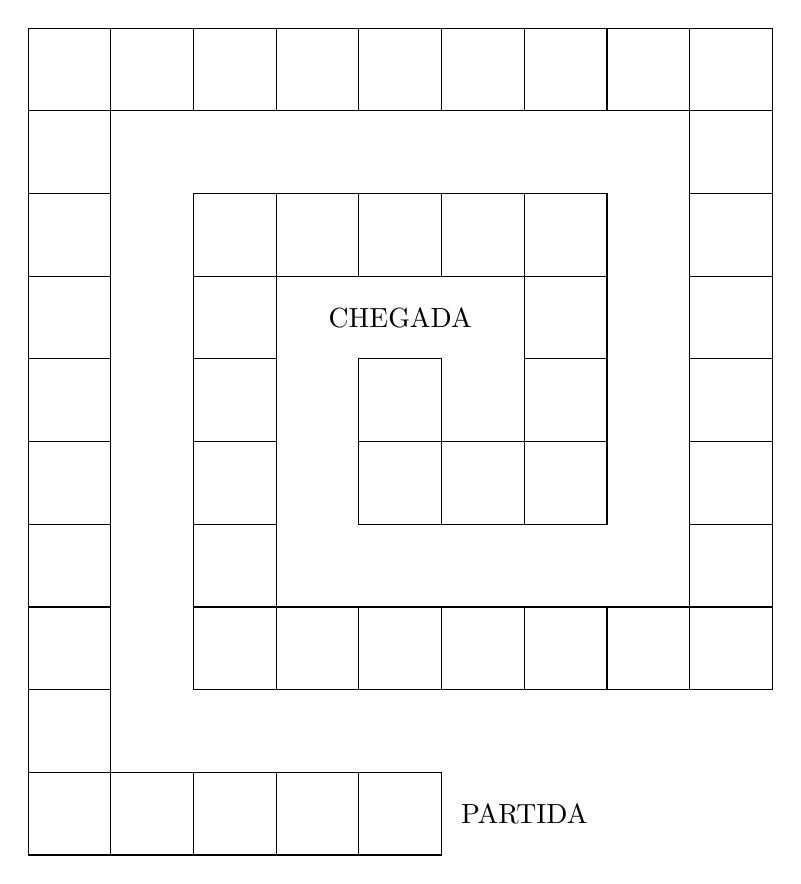
\begin{tikzpicture}[x=1.5cm,y=1.5cm, scale=.7]
\draw (4,0) rectangle (5,1);
\draw (3,0) rectangle (4,1);
\draw (2,0) rectangle (3,1);
\draw (1,0) rectangle (2,1);
\draw (0,0) rectangle (1,1);
\draw (0,1) rectangle (1,2);
\draw (0,2) rectangle (1,3);
\draw (0,3) rectangle (1,4);
\draw (0,4) rectangle (1,5);
\draw (0,5) rectangle (1,6);
\draw (0,6) rectangle (1,7);
\draw (0,7) rectangle (1,8);
\draw (0,8) rectangle (1,9);
\draw (0,9) rectangle (1,10);
\draw (1,9) rectangle (2,10);
\draw (2,9) rectangle (3,10);
\draw (3,9) rectangle (4,10);
\draw (4,9) rectangle (5,10);
\draw (5,9) rectangle (6,10);
\draw (6,9) rectangle (7,10);
\draw (7,9) rectangle (8,10);
\draw (8,9) rectangle (9,10);
\draw (8,8) rectangle (9,9);
\draw (8,7) rectangle (9,8);
\draw (8,6) rectangle (9,7);
\draw (8,5) rectangle (9,6);
\draw (8,4) rectangle (9,5);
\draw (8,3) rectangle (9,4);
\draw (8,2) rectangle (9,3);
\draw (7,2) rectangle (8,3);
\draw (6,2) rectangle (7,3);
\draw (5,2) rectangle (6,3);
\draw (4,2) rectangle (5,3);
\draw (3,2) rectangle (4,3);
\draw (2,2) rectangle (3,3);
\draw (2,3) rectangle (3,4);
\draw (2,4) rectangle (3,5);
\draw (2,5) rectangle (3,6);
\draw (2,6) rectangle (3,7);
\draw (2,7) rectangle (3,8);
\draw (3,7) rectangle (4,8);
\draw (4,7) rectangle (5,8);
\draw (5,7) rectangle (6,8);
\draw (6,7) rectangle (7,8);
\draw (6,6) rectangle (7,7);
\draw (6,5) rectangle (7,6);
\draw (6,4) rectangle (7,5);
\draw (5,4) rectangle (6,5);
\draw (4,4) rectangle (5,5);
\draw (4,5) rectangle (5,6);
\draw (6,0.5) node[]{PARTIDA};
\draw (4.5,6.5) node[]{CHEGADA};
\end{tikzpicture}
\end{center}

Seu grupo também receberá peões que identificarão as posições dos jogadores na trilha. Cada jogador deve escrever o seu nome no peão (na imagem a seguir, o peão está com o nome ``Antônio'').
\begin{center}
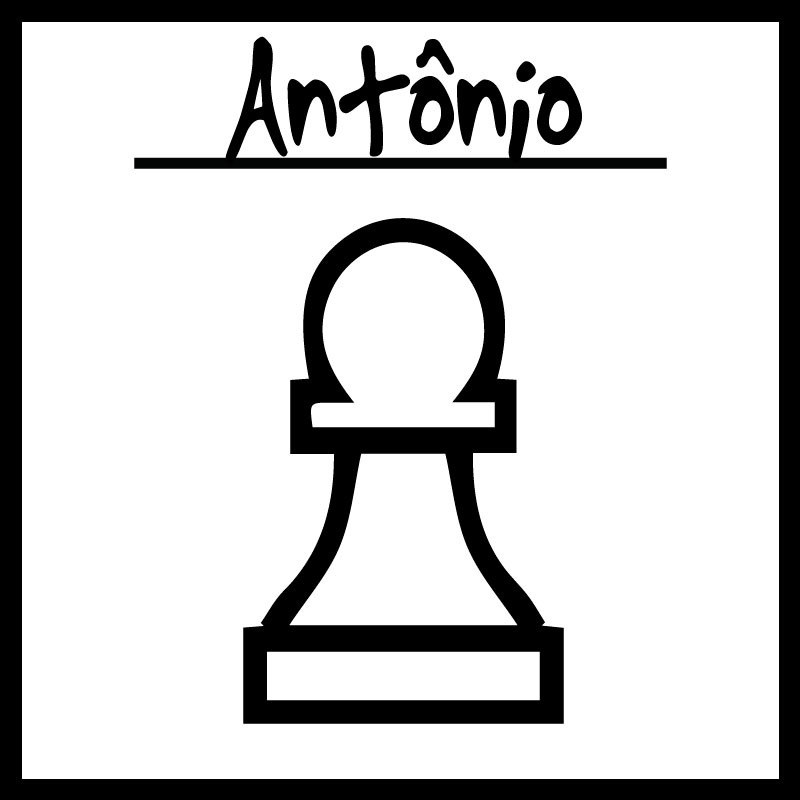
\includegraphics[width=50pt, keepaspectratio]{caminho-peao.jpeg}
\end{center}
O dado pode ser usado para decidir a ordem de jogada. As regras do jogo são as seguintes:


$1^{\textrm{\underline{o}}}$ No desenvolvimento do jogo, cada jogador lança o dado duas vezes. Esses lançamentos determinam a fração que correspondente ao movimento que o jogador fará: o primeiro lançamento registra o denominador da fração e o segundo o numerador. Assim, por exemplo, se o primeiro lançamento do dado resulta no número 12 e o segundo lançamento resulta no número 10, a fração correspondente é $\frac{10}{12}$. Outro exemplo: se o número do primeiro lançamento do dado é $6$ e o número do segundo lançamento é $3$, a fração correspondente é $\frac{3}{6}$. Mais um exemplo: se o número do primeiro lançamento do dado é $5$ e o número do segundo lançamento é $7$, a fração correspondente é $\frac{7}{5}$.

$2^{\textrm{\underline{o}}}$ Se a fração obtida com o lançamento dos dados for equivalente a uma fraçào de denominador 12, ou seja, a certa quantidade de doze avos, o peão ``caminha'' essa quantidade de passos. Caso contrário, ele não sai do lugar que está e passa a vez para o próximo jogador. Assim, por exemplo: se a fração obtida for $\frac{10}{12}$, seu peão andará 10 casas. Se a fração obtida for $\frac{3}{6}$, seu peão andará $6$ casas, pois $\frac{3}{6} = \frac{6}{12}$. Se a fração obtida for $\frac{7}{5}$, seu peão permanecerá na casa em que está e você passará a vez.

$3^{\textrm{\underline{o}}}$ Vence o jogo aquele jogador que, em primeiro lugar, atingir o ponto de chegada.

Depois de jogar algumas vezes responda às questões a seguir.


\begin{enumerate}
 \item Quantos passos um jogador deu se ele obteve nos dois lançamentos respectivamente os seguintes números:

 \noindent \begin{tabular}{m{.17\textwidth}m{.17\textwidth}m{.17\textwidth}m{.17\textwidth}m{.17\textwidth}}
1º) 12 e 7?  & 2º) 6 e 5? & 3º) 8 e 6? & 4º) 8 e 7? & 5º) 9 e 12? \\
6º) 7 e 8? & 7º) 11 e 4? & 8º) 1 e 1? & 9º) 6 e 3? & 10º) 3 e 6?
\end{tabular}

\item   Em 5 rodadas consecutivas, o primeiro jogador sorteou as frações  $\frac{7}{12}$, $\frac{10}{9}$, $\frac{1}{3}$, $\frac{3}{2}$e  $\frac{12}{6}$. Já o segundo jogador, nessas 5 rodadas, deu ao todo 47 passos. Ao final dessas rodadas, qual deles está a frente?
\end{enumerate}

\ifdefined\prof
\begin{solucao}

\begin{enumerate}
\item 1º) 7 casas. 2º) 10 casas. 3º) 9 casas. 4º) Fica parado e passa a vez. 5º) 16 casas. 6º) Fica parado e passa a vez. 7º) Fica parado e passa a vez. 8º) 12 casas. 9º) 6 casas.
10º) 24 casas.

\item O primeiro jogador andou $7 + 0 + 4 + 18 + 24 = 53$ casas. Portanto, o primeiro jogador está na frente e venceu o jogo.
\end{enumerate}


\end{solucao}
\fi

\end{document}